\chapter{Berechnung der Potenzialfelder}

Die Grundlage der Pfadplanung zu einem Zielpunkt bildet in dieser Implementierung die \textit{Potenzialfeldmethode}:
Der Konfigurationsraum entspricht einem skalaren \textit{Potenzialfeld}, wobei jede Koordinate eine potenzielle Energie $U(\texttt{x}, \texttt{y}, \texttt{rotation})$ besitzt, ausgedrückt durch eine reelle Zahl.
Je Höher die potenzielle Energie einer Koordinate, desto weiter ist der Punkt auf dem aktuellen Pfad vom Ziel entfernt.
Die Berechnung des Potenzialfelds $\texttt{potential[rotation][y][x]} = U(\texttt{x}, \texttt{y}, \texttt{rotation})$ erfolgt mit \textit{Potenzialfunktionen}. \cite{yujiang.2017}

\vspace*{0.2cm}
\section{Anziehende \& Abstoßende Potenziale} \label{sec:attr-repul-pot}

Khatib schlug 1986 vor, das Potenzialfeld in Analogie zu Gravitationsfeldern zu berechnen \cite{khatib.1985}. Der zu erreichende Zielpunkt wirkt mit einem \textit{anziehenden} (engl. \textit{attractive}) Potenzial auf eine Koordinate (\texttt{y}, \texttt{x}). Dieses Potenzial ist in allen Rotationsebenen gleich:
\vspace*{0.25cm}
\begin{equation*}
U_{Attr, Ziel}(\texttt{x}, \texttt{y}) = \sqrt{(\texttt{y} - \texttt{y}_{Ziel})^2 + (\texttt{x} - \texttt{x}_{Ziel})^2}
\end{equation*}

%\vspace*{-0.1cm}
Bei den getesteten Implementierungsszenarien wurden bessere Ergebnisse festgestellt, wenn das anziehenden Potenzial erst normiert und anschließend gewichtet wird. Mit $\texttt{attraction\_weight} = 1$ hat das anziehende Potenzial einen Wertebereich von $[0;1]$. Mit  $\texttt{attraction\_weight} < 1$ wird die obere Grenze des Wertebereichs verringert, mit $\texttt{attraction\_weight} > 1$ vergrößert:
\vspace*{0.3cm}
\begin{equation*}
U_{Attr, Ziel}(\texttt{x}, \texttt{y})_{norm} = \frac{U_{Attr, Ziel}(\texttt{x}, \texttt{y})}{\max \{ U_{Attr, Ziel}\}} * \texttt{attraction\_weight} 
\end{equation*}

%\vspace*{-0.1cm}
Die Hindernisse im Konfigurationsraum wirken auf jede Koordinate (\texttt{x}, \texttt{y}, \texttt{rotation}) mit einem \textit{abstoßendem} (engl. \textit{repulsive}) Potenzial. Dazu zählen auch die Hindernisse aus der benachbarten Rotationsebene \texttt{((rotation+1) \% rotations)} sowie \texttt{((rotation-1) \% rotations)}. Mit $\texttt{repulsion\_weight}=0$ hat das abstoßende Potenzial einen Wertebereich von $[0;1]$. Werte $\texttt{repulsion\_weight} > 0 $ verringern die obere Grenze des Wertebereichs gegen $0$: \cite{schweiger.2023}
\vspace*{0.25cm}
\begin{equation*}
\hspace*{-0.075\linewidth}
\resizebox{1.15\linewidth}{!}{
  $ U_{Repul, Hindernis}(\texttt{x}, \texttt{y}, \texttt{rotation}) = \frac{1}{\texttt{repulsion\_weight} + \sqrt{(\texttt{y} - \texttt{y}_{Hindernis})^2 + (\texttt{x} - \texttt{x}_{Hindernis})^2 + (\texttt{rotation} - \texttt{rotation}_{Hindernis})^2}}
$}
\hspace*{-0.075\linewidth}
\end{equation*}

\vspace*{0.05cm}
Yujiang und Huilin definieren das abstoßende Potenzial einer Koordinate als kleinsten Abstand zu allen Hindernissen \cite{yujiang.2017}:
\vspace*{0.3cm}
\begin{equation*}
U_{Repul}(\texttt{x}, \texttt{y}, \texttt{rotation}) = \min_{\forall \,\,Hindernis \,\,\in \texttt{ occupancy\_grid}} \{ U_{Repul, Hindernis}(\texttt{x}, \texttt{y}, \texttt{rotation}) \}
\end{equation*}

%\vspace*{-0.1cm}
Die gesamte potenzielle Energie einer Koordinate entspricht der Kombination beider Potenziale. In dieser Implementierung wurden anziehendes und abstoßendes Potenzial gemäß Khalib addiert \cite{khatib.1985}:
\vspace*{0.25cm}
\begin{equation*}
U(\texttt{x}, \texttt{y}, \texttt{rotation}) = U_{Attr, Ziel}(\texttt{x}, \texttt{y})_{norm} + U_{Repul}(\texttt{x}, \texttt{y}, \texttt{rotation})
\end{equation*}
\begin{figure}[H]
	\centering
	\footnotesize
	\centerline{\resizebox{1\linewidth}{!}{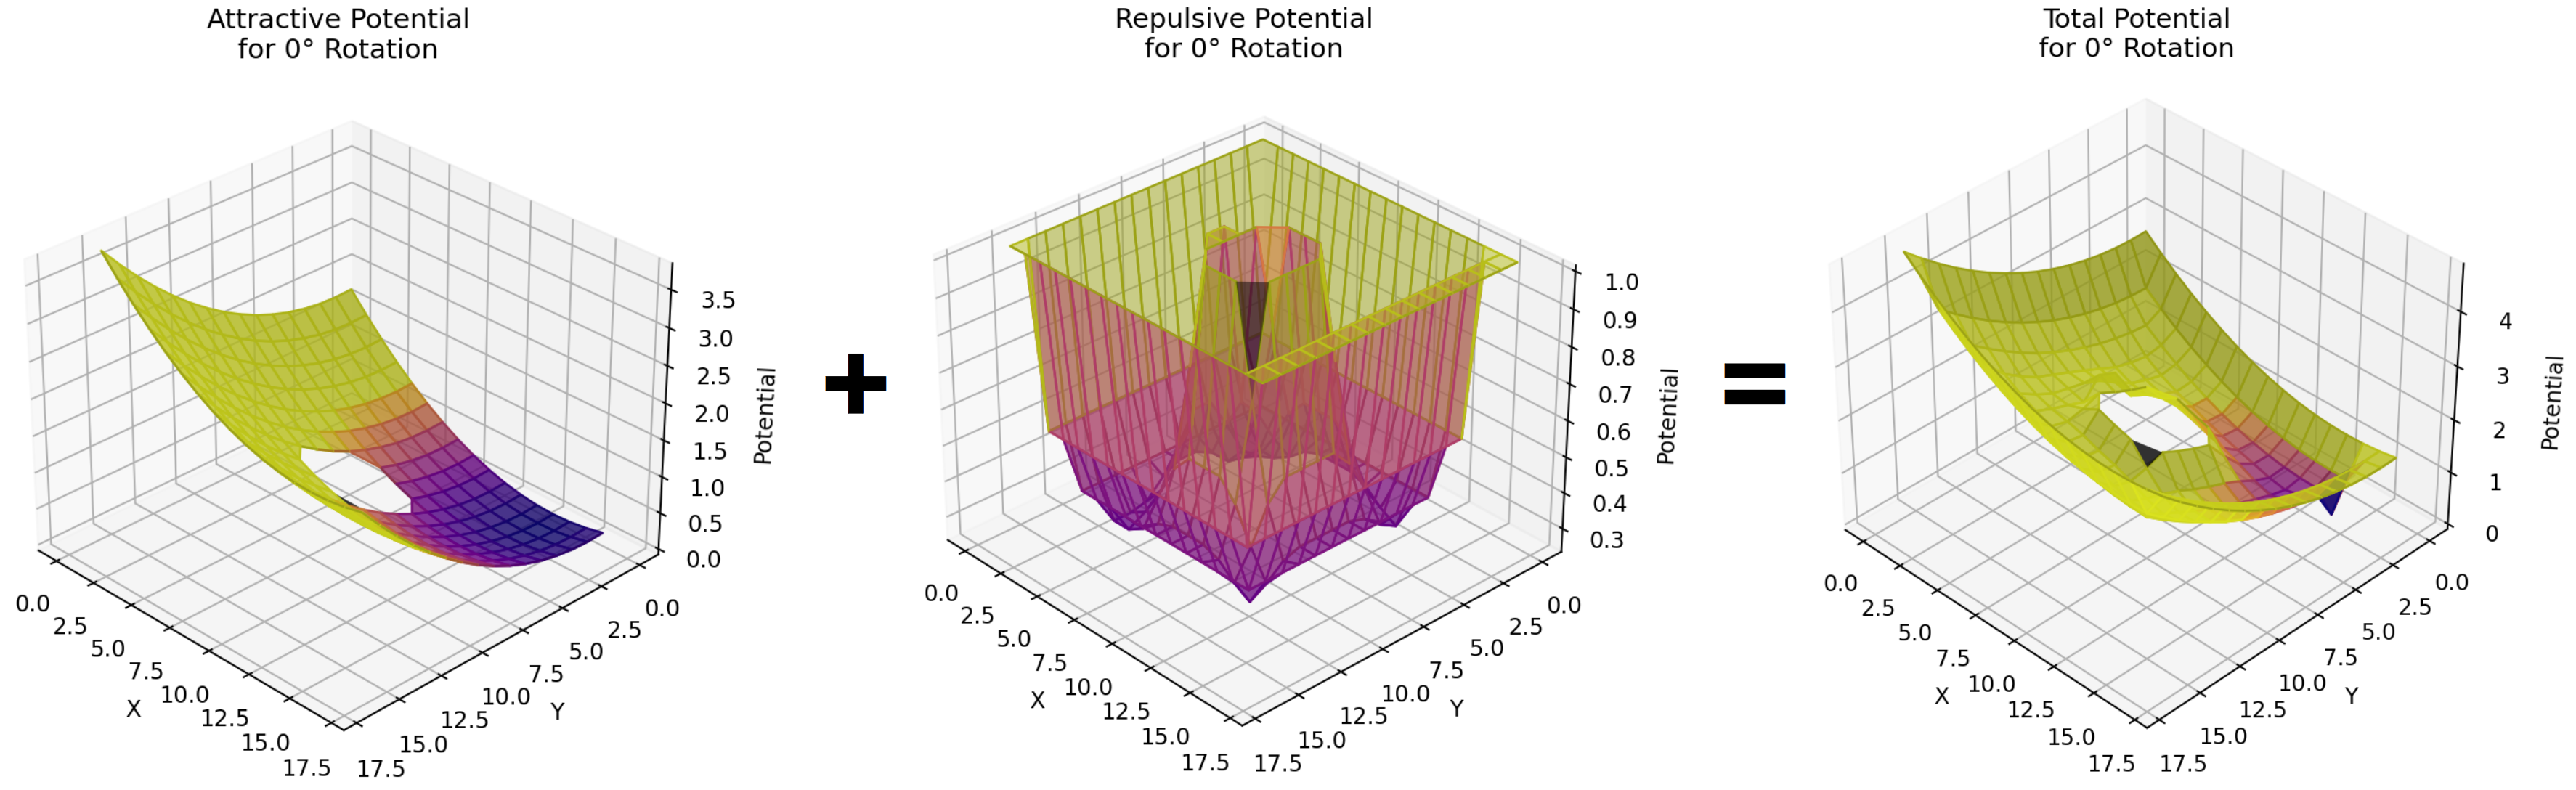
\includegraphics{bilder/total-potential-computation.png}}}
	\caption{Die Berechnung des Gestamtpotenzial für die $0$°-Rotationsebene des Konfigurationsraums mit \texttt{attraction\_weight=5} und \texttt{repulsion\_weight=0}.}
\end{figure}

\vspace*{0.2cm}
\section{Wavefront Potenziale}

Choset stellt eine Potenzialfunktion unter Verwendung der Breitensuche ausgehend vom Zielpunkt vor. Beim sogenannten \textit{Wavefront-Algorithmus} entsprechen die Koordinaten des Konfigurationsraums den Knoten der Breitensuche, wobei jeder besuchte Knoten das pro Breitensuchenebene streng monoton steigende Potenzial erhält: \cite{choset.2007}
\vspace*{0.1cm}
\begin{algorithm}
\caption{Wavefront-Algorithmus}
	\begin{algorithmic}[1]
  \State \textbf{Initialisierung:}
  \State \hspace{\algorithmicindent} Jeder Punkt $U(\texttt{x}, \texttt{y}, \texttt{rotation}) = 0$
  \State \hspace{\algorithmicindent} Warteschlange $Q := \{((\texttt{x}_{Ziel}, \texttt{y}_{Ziel}, \texttt{rotation}_{Ziel}), 2)\}$
		\vspace*{0.3cm}
  \While{$Q \neq \emptyset$}
      \State $((\texttt{x}, \texttt{y}, \texttt{rotation}), \texttt{potential}) \gets Q$
      \State $U(\texttt{x}, \texttt{y}, \texttt{rotation}) = \texttt{potential}$
      \State Nachbarn $N := \{(\texttt{x-1}, \texttt{y}, \texttt{rotation}), (\texttt{x+1}, \texttt{y}, \texttt{rotation}), ... (\texttt{x}, \texttt{y}, \texttt{(rotation-1) \% rotations})\}$
      \For{$(\texttt{x}_{Nachbar}, \texttt{y}_{Nachbar}, \texttt{rotation}_{Nachbar}) \gets N$}         
          \If{$0 \leq \texttt{x}_{Nachbar} < \texttt{occupancy\_grid\_width}$ \\
              \hspace*{\algorithmicindent}\hspace*{\algorithmicindent} \textbf{and} $0 \leq \texttt{y}_{Nachbar} < \texttt{occupancy\_grid\_height}$ \\
              \hspace*{\algorithmicindent}\hspace*{\algorithmicindent} \textbf{and} $ \texttt{computational\_space}[\texttt{rotation}_{Nachbar}][\texttt{y}_{Nachbar}][\texttt{x}_{Nachbar}] = \texttt{True}$}
              \State $((\texttt{x}_{Nachbar}, \texttt{y}_{Nachbar}, \texttt{rotation}_{Nachbar}), \texttt{potential + 1}) \rightarrow Q$
          \EndIf
      \EndFor
  \EndWhile
	\end{algorithmic}
\end{algorithm}

\newpage
Somit breitet sich ausgehend vom Zielpunkt als Quelle das ansteigende Potenzial bildlich als \textit{Wellenfront} im Konfigurationsraum aus.
Koordinaten in Hindernisnähe erhalten auf entgegengesetzter Seite der Ausbreitungsrichtung höhere Potenziale.

\begin{figure}[H]
	\centering
	\footnotesize
	\centerline{\resizebox{1\linewidth}{!}{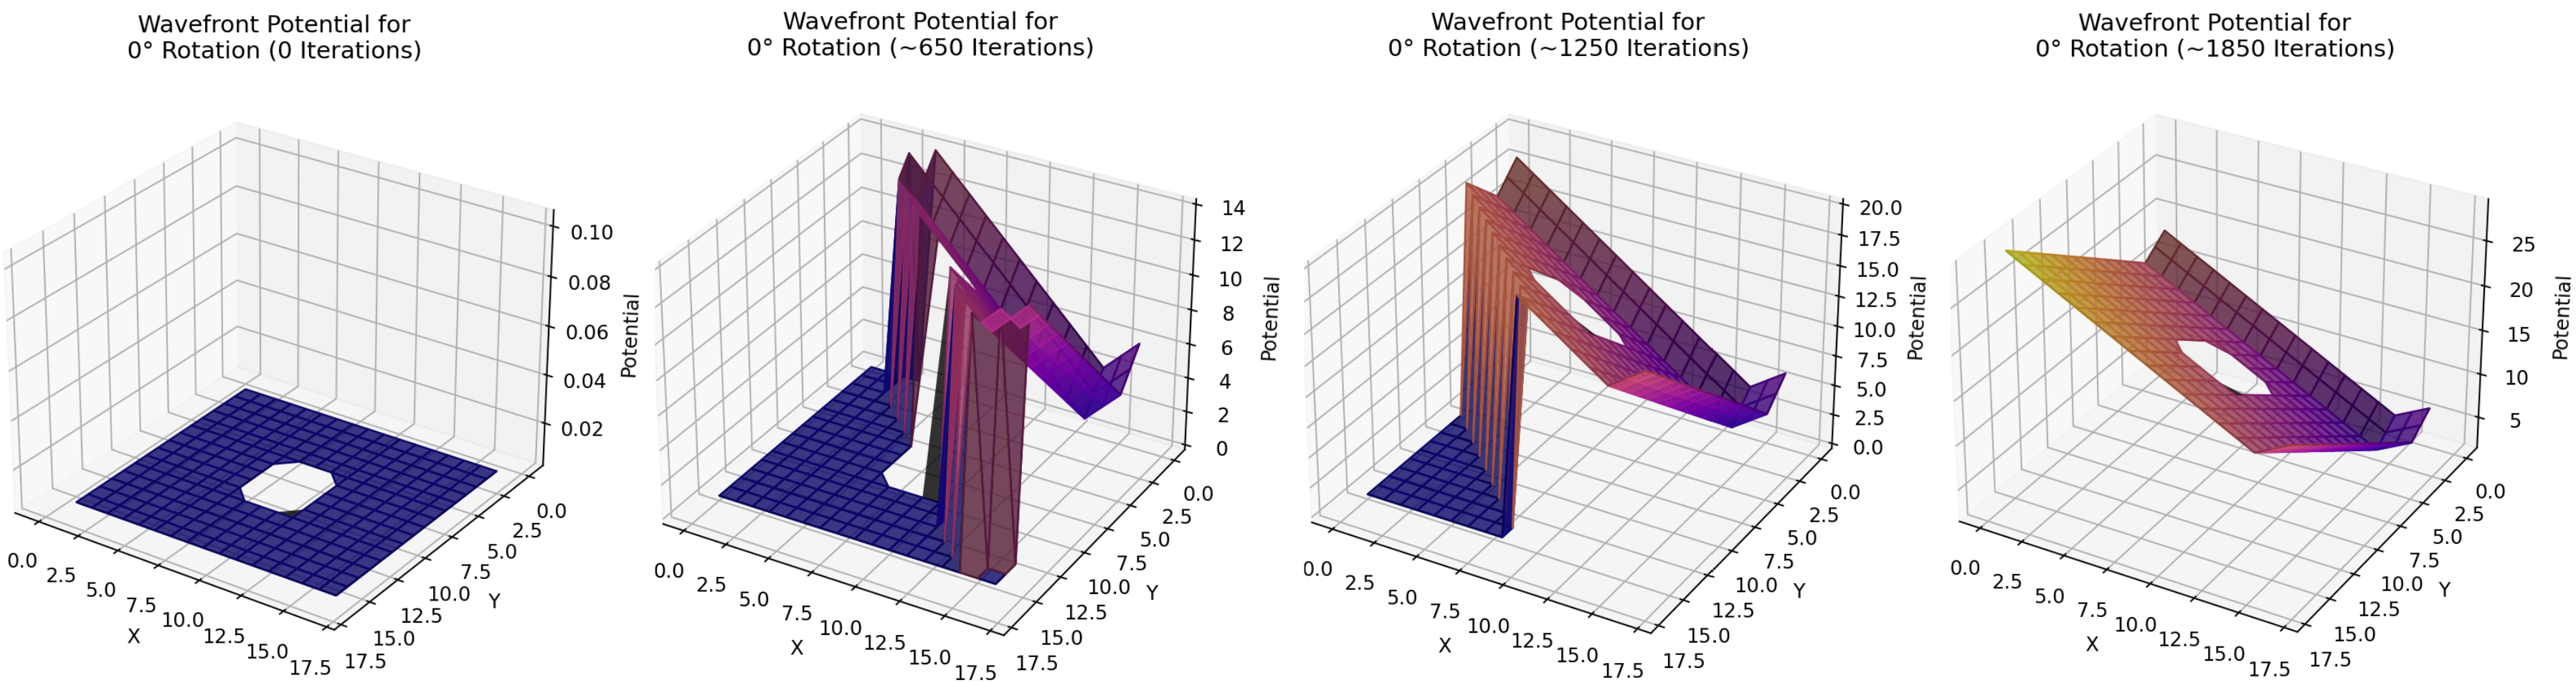
\includegraphics{bilder/wavefront.png}}}
	\caption{Die Berechnung des Gestamtpotenzial für die $0$°-Rotationsebene des Konfigurationsraums mit $\texttt{attraction\_weight}=5$ und $\texttt{repulsion\_weight}=0$.}
\end{figure}

\vspace*{1cm}
Unabhängig von der gewählten Potenzialfunktion wird das Potenzialfeld im dreidimensionalen Konfigurationsraum für jede Rotationsebene berechnet.
Somit hat das Potenzialfeld die gleichen Dimensionen wie der Konfigurationsraum:

\begin{figure}[H]
	\centering
	\footnotesize
	\centerline{\resizebox{1\linewidth}{!}{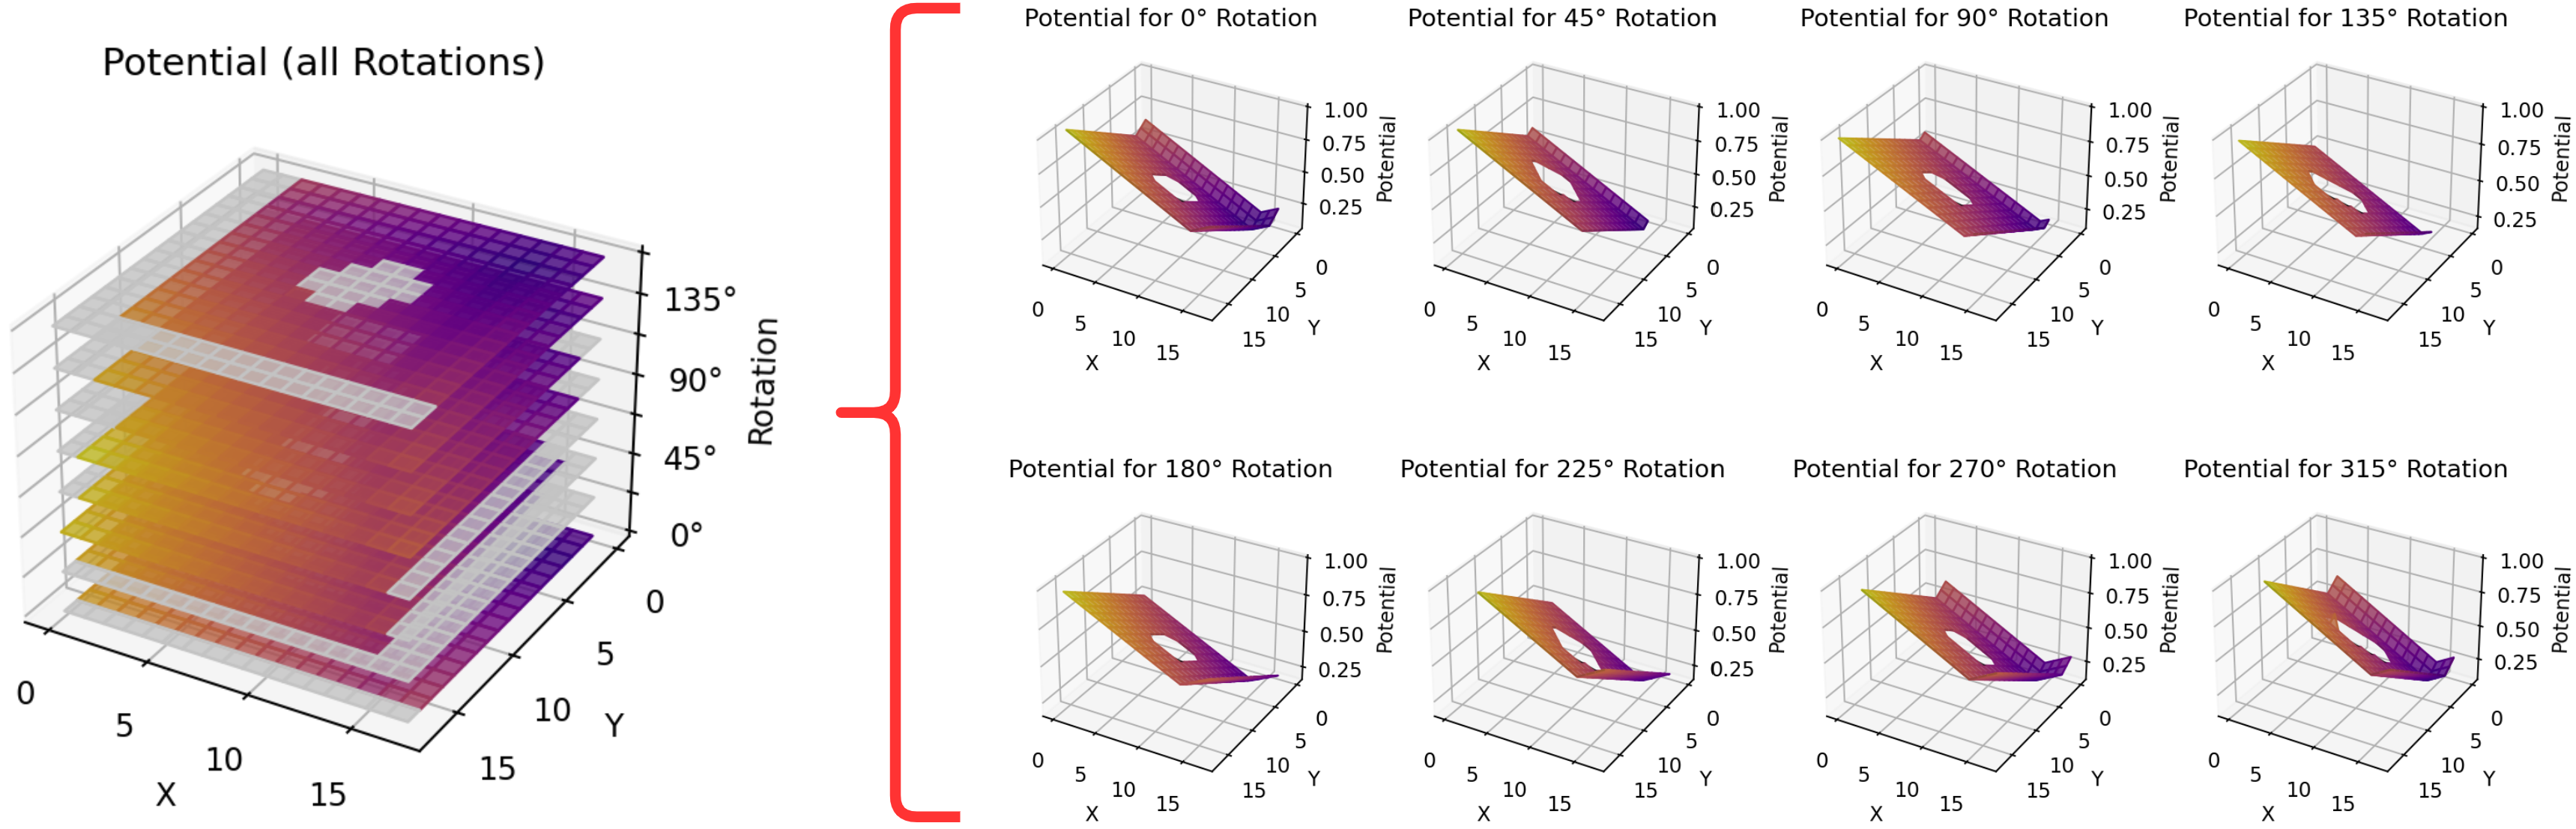
\includegraphics{bilder/potential-stacked-computed.png}}}
	\caption{Das Potenzialfeld wird im dreidimensionalen Konfigurationsraum berechnet.}
\end{figure}


